\chapter{Styrhandske}
\begin{figure}[htb]
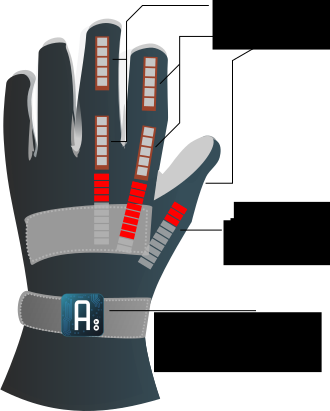
\includegraphics[height=0.5\textheight]{img/kontrollhandske}
\caption{Konceptskiss över styrhandsken. Röda ledlampor indikerar hur högt }
\end{figure}
%Detta är intro. Det ska inte vara några detaljer här, bara översiktligt!
% Konvention: styrhandske, inte reglerhandske eller kontrollhanske

För att intuitivt reglera robothanden används en tunn handske som användaren bär på sin hand. På handskens tumme, långfinger och pekfinger finns det två flexsensorer vardera som följer användarens hand och ändrar resistans beroende på hur mycket de böjs. Resistansen samplas av en mikrokontroller, som efter filtrering trådlöst sänder styrsignaler till robothanden.
Robothanden sänder i sin tur trycket från dess fingrar till styrhandsken. Trycket återkopplas till användaren genom att fler ledlampor på handen tänds ju större trycket är.


\section{Konstruktion}
\comment{Emil: Skriv om handens fysiska konstruktion}

\section{Elektronik}
\comment{Kanske något enkelet schema för hur det är uppkopplat}


\section{Mikrokontroller}
För styrhandsken används en \emph{Arduino Micro}, en 16 bitars AVR mikroprocessor.
Mikrokontrollen

\begin{figure}[htb]
\includegraphics[width=0.3\textwidth]{img/arduino_micro}
\caption{Ardunio Micro. Används för kontrollhandsken.}
\end{figure}


\section{Trådlös kommunikation}
För att möjliggöra kommunikation trådlöst mellan styrhandsken och robothanden används två prototyp-versioner av \emph{Bluetooth Mate Silver}. Enheten är godkänd för Bluetooth klass 2, vilket bl a innebär låg strömförbrukning (genomsnittligt 2.5mW vid aktiv användning) och överföringar på upp till 20m, vilket anses vara tillräckligt för att klara kravet på 5m i praktiska förhållanden.

Bluetooth-protokollet är ett paketförmedlande nätverk, vilket innebär att information skickas i diskreta paket. Varje paket innehåller metadata
\footnote{Data som beskriver information, som mottagaradress och felkorrigerande kod}
och \emph{payload}
\footnote{Datan i sig som ska överföras}.
Bluetooth-enheten har en överföringskapacitet på 115200bps\footnote{bits per second}, inkluderat metadata.


De två bluetoothmodulerna är programmerade att automatiskt ansluta till varandra när de är inom räckhåll, och återuppta en eventuellt förlorad anslutning.


\subsection{Säkerhet}
För att skydda mot otillåten kontroll och avlyssning av styrsignalerna mellan kontrollhandsken används kryptering.
Bluetooth definierar ett säkerhetsprotokoll där enheter utbyter symmetriska krypteringsnycklar \footnote{128 bitars med vår enhet.} antingen med hjälp av en dynamisk ``parningsprocess'', där användaren kontrollerar pinkoder vid första användningen, eller att nycklarna manuellt. 

Bluetooth är en industristandard vilket leder till att säkerheten är väl testad och beprövad till den mån att den kan anses vara fullgod för projektet, och om industriella tillämpningar i framtiden skulle var önskvärt \cite{btsec}.

\subsection{Integritet och paketförlust}
Data som överförs trådlöst kan korrumperas av t ex elektromagnetisk strålning. Utan integritetskontroll kan det leda till att felaktiga kommandon utförs, som att t ex ett för hårt tryck mosar en tomat.
Sändarmodulen räknar ut en CRC-kod\footnote{Cycle Redundancy Check --- En felkorrigerande kod som framställs genom binär polynomdivision} baserat på datan som ska skickas, och inkluderar den i slutat av bluetooth-paketet. 
Mottagarmodulen i sin tur upprepar uträkningen på datan som tas emot, och jämför det med CRC-koden. Om de inte är ekvivalenta ignoreras paketet eftersom datan då är felaktig.




\begin{figure}[ht]
\includegraphics[width=0.3\textwidth]{img/bluetooth_mate_silver.jpg}
\caption{Bluetooth Mate Silver enhet.}
\end{figure}


\section{Signalbehandling}
Från flexsensorerna samplas en varierande analog spänning med en frekvens på 100 Hz. Signalen diskretireras sedan till upplösning av 10 bitar. I uppmätta mätvärdet finns det diverse störningar. Det är inte önskvärt att störningarna överförs till robothanden, eftersom servomotorerna i robothanden då konstant skulle ändra läge, vilket leder till en hackig upplevelse för användaren, slitage på servomotorerna, och extra strömförbrukning.

\begin{figure}[htb]
\includegraphics{img/filter/flex_raw.pdf}
\caption{De sex flexsensorerna uppmätta under 8.0s med en samplingsfrekvens på 100Hz när handen greppar ett objekt.}
\label{fig:rawflex}
\end{figure}

\begin{figure}[htb]
\includegraphics{img/filter/flex_fourier.pdf}
\caption{Diskret fouriertransform av signalerna från figur~\ref{fig:rawflex}.}
\end{figure}


\begin{figure}[htb]
\includegraphics{img/filter/flex_filtered.pdf}
\caption{Signalerna från figur~\ref{fig:rawflex} filtrerade med ett Butterworth-filter av första ordningen med en brytningsfrekvens på $f=\unit[15]{Hz}$.}
\end{figure}



För att filtera signalen används ett \emph{Butterworth-filter} av första ordningen. Butterworth filter filterar


\section{Algoritmer}
Här presenteras de styralgortimter som bestämmer hur handen beter sig när den följer användarens input samt identifierar och greppar objekt. 


\section{Objektidentifiering}
\begin{figure}[H]
EN BILD SOM FÖRKLARAR DETTA, SAMT VILKA OBJEKT VI VALT ATT identifierar och hur vi gör det...
\caption{Beskrivning}
\end{figure}
Antaganden: Servona står i önskat läge, det vill säga tidsfördröjningen som uppstår då servona skall vrida sig från godtycklig position till den önskade antags vara så liten vid normalt användande att den kan försummas. Då ingen mätning av servonas verkliga position görs, är den enda informationen om fingrarnas lägen det önskade servoläget. 

FIXA FLÖDESSSCHEMA OCH ETT ARDUINO PROGRAM Känner av tryck (över visst gränsvärde) på tumme och motstående finger->, lagrar användarens input läge då detta inträffar ( för att när användaren går utanför detta igen (öppnar sin hand) så skall handen återgår till att följa användaren) -> beräknar avståndet mellan sensorerna-> checkar av avståndet mot en lista av fördefinerade objekt som innehåller , storlek och önskat trycksensorvärde med en +/-tolerans för att inte handen ska stå och flippa som en tok för att uppnå EXAKT rätt värde-> TADAA!!-> när användaren öppnar sina fingrar utanför ``kontaktläget'' följer handen efter igen...
Mer teksti
